\chapter{Objetos Extendidos}

\section{Introducción}

En esta sección estudiaremos los llamados \textbf{objetos extendidos} y
su formalismo. Objetos de este tipo son sólidos, cuerdas, membranas,
líquidos, etc.

Un objeto extendido es aquel que no corresponde a una partícula puntual:
abandonamos la descripción de la forma $q^i(t)$, que describe una curva
en el espacio de configuración, y la reemplazamos por un objeto que se
extiende en más de una dimensión.

El caso de mayor interés corresponde a la llamada \textbf{teoría de
campos}. Este concepto lo introdujo Faraday (1791--1867) para interpretar
las leyes que rigen las acciones entre cargas, corrientes eléctricas e
imanes: el concepto de campo se introdujo para interpretar la acción a
distancia de acuerdo con las ideas filosóficas de Aristóteles, la
\emph{contigüidad} de las interacciones entre las distintas partes del
Universo.

\subsection{La cuerda vibrante}

Comencemos con el estudio de una cuerda vibrante. Como no conocemos el
formalismo de objetos extendidos, debemos partir con la teoría de
Newton. Para acomodar la segunda ley de Newton a la cuerda debemos
recurrir al cálculo infinitesimal y dividimos la cuerda en elementos
infinitesimales de masa $dm$ tales que
\[
dm\,\vec a = d\vec T = \vec T(x+dx) - \vec T(x),
\]
donde $d\vec T$ es un diferencial de la tensión.

\begin{center}
\begin{tikzpicture}[scale=1]
  \draw[thick] (0,0) .. controls (2,0.8) and (4,-0.8) .. (6,0);
  \draw[-Stealth] (2.05,0.75) -- (1.3,1.4) node[above] {\footnotesize$\vec T(x)$};
  \draw[-Stealth] (3.95,-0.75) -- (4.7,-1.3) node[below] {\footnotesize$\vec T(x+dx)$};
  \draw[dashed] (0,0) -- (6,0);
  \fill (2,0.8) circle (1.2pt) node[below] {\footnotesize$x$};
  \fill (4,-0.8) circle (1.2pt) node[above] {\footnotesize$x+dx$};
\end{tikzpicture}
\end{center}

De acuerdo con el sistema coordenado elegido,
\[
dm\, a_x = dT_x, \qquad dm\, a_z = dT_z .
\]
Queremos que la cuerda oscile solo a lo largo del eje $z$, es decir, no
hay movimiento en el eje $x$, entonces $a_x=0$, por lo que
\[
dT_x = T(x+dx)\cos\alpha(x+dx) - T(x)\cos\alpha(x),
\]
donde $T(x)$ es el módulo de la tensión $\vec T(x)$.

\begin{proposicionc}
La componente de la tensión sobre el eje $x$ es constante:
$T(x)\cos\alpha(x) = T = \text{constante}$.
\end{proposicionc}

\begin{proof}
Haciendo un desarrollo en serie de Taylor a primer orden en $dx$,
\[
dT_x = \left(T(x)+\frac{dT}{dx}dx\right)\left(\cos\alpha(x)+
\frac{d\cos\alpha(x)}{dx}dx\right) - T(x)\cos\alpha(x) =
\frac{d}{dx}\big(T(x)\cos\alpha(x)\big)\, dx = 0,
\]
donde en el último paso usamos $a_x=0$. Por lo tanto $T(x)\cos\alpha(x)$
es la misma constante en cada punto del eje $x$. \qedhere
\end{proof}

La componente sobre el eje $z$ es
\[
dm\,a_z = T(x+dx)\sin\alpha(x+dx) - T(x)\sin\alpha(x) = T\big(\tan
\alpha(x+dx)-\tan\alpha(x)\big),
\]
donde se usó $T(x)\cos\alpha(x)=T=\text{constante}$ para reescribir cada
término como $T(x)\cos\alpha(x)\tan\alpha(x)=T\tan\alpha(x)$.

La aceleración de la cuerda debiera estar dada por $a_z=d^2z(t)/dt^2$.
Sin embargo, la cuerda es un objeto extendido, por lo que cada punto de
la cuerda puede tener aceleraciones distintas: la aceleración varía a lo
largo del eje $x$, y por lo tanto la coordenada $z$ no solo varía con el
tiempo sino también con la coordenada $x$, esto es $z=z(t,x)$. Entonces
\[
a_z = \frac{\partial^2 z}{\partial t^2}(t,x).
\]

Además, $\tan\alpha(x) = \partial z(t,x)/\partial x$ es la pendiente de
la curva que corresponde a la cuerda oscilante (la variable $\alpha$
también depende del tiempo, $\alpha(t,x)$). Entonces
\[
dm\, \frac{\partial^2 z(t,x)}{\partial t^2} = T\left(\frac{\partial
z}{\partial x}(t,x+dx) - \frac{\partial z}{\partial x}(t,x)\right) =
T\,\frac{\partial^2 z(t,x)}{\partial x^2}\, dx .
\]

\begin{definicion}[Densidad de masa lineal]
La masa está distribuida a lo largo de una curva, que es la cuerda, por
lo que definimos la \textbf{densidad de masa lineal} como
$\lambda = dm/dx$, que consideraremos homogénea ($\lambda=$ constante).
\end{definicion}

\begin{proposicionc}[Ecuación de la cuerda vibrante]
La cuerda vibrante satisface la ecuación diferencial parcial lineal de
segundo orden
\[
\lambda\, \frac{\partial^2 z(t,x)}{\partial t^2} = T\,
\frac{\partial^2 z(t,x)}{\partial x^2} .
\]
\end{proposicionc}

\subsection{Generalización a la membrana vibrante}

La ecuación de la cuerda vibrante se generaliza fácilmente a la ecuación
de una membrana vibrante, es decir, pasamos de un objeto unidimensional a
uno bidimensional. Al igual que con la cuerda, seccionamos la membrana en
pequeñas áreas infinitesimales de masa $d^2m$, con $z=z(t,x,y)$, y se
obtiene
\[
d^2m\, \frac{\partial^2 z}{\partial t^2} = T\,\frac{\partial^2
z}{\partial x^2}\, dx\,dy + T\, \frac{\partial^2 z}{\partial y^2}\,
dx\,dy .
\]

\begin{definicion}[Densidad de masa superficial]
Se define la densidad de masa superficial como $\sigma = d^2m/(dx\,dy)$,
que asumiremos homogénea, $\sigma=$ constante.
\end{definicion}

Por lo tanto,
\[
\sigma\, \frac{\partial^2 z}{\partial t^2} = T\left(\frac{\partial^2
z}{\partial x^2} + \frac{\partial^2 z}{\partial y^2}\right).
\]
Esto se generaliza, como veremos, a la forma
\[
\frac{1}{v_p^2}\, \frac{\partial^2\phi}{\partial t^2} =
\frac{\partial^2\phi}{\partial x^2} + \frac{\partial^2\phi}{\partial
y^2} + \frac{\partial^2\phi}{\partial z^2},
\]
donde $v_p$ es la rapidez de propagación.

\begin{observacion}
En ambos casos (cuerda y membrana), una coordenada no solo depende del
tiempo, sino que se vuelve dependiente de las otras coordenadas
espaciales. Esto es característico de los objetos extendidos en mecánica
clásica. En las ecuaciones de Navier--Stokes, que describen los fluidos,
la magnitud física a encontrar es la velocidad, que depende del tiempo y
de las coordenadas cartesianas, $\vec u(t,x,y,z)$.
\end{observacion}

\subsection{Campos versus coordenadas}

En teoría de campos, la variable física a determinar no es una
coordenada, sino una variable que define un espacio distinto del espacio
físico donde se mueven los objetos. Por ejemplo, en la teoría
electromagnética los campos que varían temporal y espacialmente son el
campo eléctrico $\vec E$ y la inducción magnética $\vec B$, que
corresponden a seis magnitudes físicas satisfaciendo ocho ecuaciones
diferenciales de primer orden (las ecuaciones de Maxwell):
\[
\vec\nabla\cdot\vec E = \frac{\rho}{\varepsilon_0}, \qquad
\frac{\partial\vec B}{\partial t} + \vec\nabla\times\vec E = 0, \qquad
\vec\nabla\times\vec B - \varepsilon_0\mu_0\frac{\partial\vec
E}{\partial t} = \varepsilon_0\mu_0\vec J, \qquad \vec\nabla\cdot\vec B
= 0.
\]
En vez de usar el campo eléctrico y magnético podemos usar los
potenciales eléctrico $\phi$ y vectorial magnético $\vec A$. Estos
potenciales pueden agruparse en un solo potencial de cuatro componentes,
llamado \textbf{cuadripotencial electromagnético}, $A^\mu = (c\phi,
A_x,A_y,A_z)$, que satisface ecuaciones de segundo orden, donde $c$ es la
rapidez de la luz. El cuadripotencial define un espacio de cuatro
dimensiones, que no corresponde al espacio físico donde se mueven los
objetos.

\subsection{El problema de Cauchy}

Volvamos a la ecuación de la cuerda vibrante,
\[
\lambda\, \frac{\partial^2 z(t,x)}{\partial t^2} = T\,\frac{\partial^2
z(t,x)}{\partial x^2}.
\]
Dividiendo por $T$ y usando análisis dimensional, $[\lambda/T] =
\text{s}^2/\text{m}^2$, definimos la \textbf{rapidez de propagación}
\[
v_p := \sqrt{\frac{T}{\lambda}},
\]
tal que la ecuación de la cuerda vibrante se escribe como
\[
\frac{1}{v_p^2}\, \frac{\partial^2 z(t,x)}{\partial t^2} =
\frac{\partial^2 z(t,x)}{\partial x^2},
\]
que es la \textbf{ecuación de onda} unidimensional con rapidez $v_p$.

\begin{proposicionc}
La solución de la ecuación de la cuerda vibrante se escribe, en forma
general, como
\[
z(t,x) = f(x-v_pt) + g(x+v_pt),
\]
donde $f(\xi)$ y $g(\xi')$, con $\xi=x-v_pt$, $\xi'=x+v_pt \in
\mathbb{R}$, son funciones arbitrarias.
\end{proposicionc}

\begin{observacion}
En la cuerda hay dos rapideces: la rapidez de oscilación a lo largo del
eje $z$, $\partial z/\partial t$, y la rapidez de propagación a lo largo
del eje $x$, $v_p$. La velocidad de propagación $v_p$ es la velocidad con
que la información de la oscilación pasa de un elemento infinitesimal de
la cuerda a otro: el elemento en el punto $x$ le transmite la
información al elemento en el punto $x+dx$, que debe oscilar.
\end{observacion}

La ecuación de la cuerda posee una derivada parcial de segundo orden en
el tiempo, por lo que al integrarla aparecen dos constantes de
integración, que se fijan a partir de \textbf{condiciones iniciales}:
\[
z(0,x) = F(x), \qquad \frac{\partial z}{\partial t}(0,x) = G(x),
\]
donde $F(x)$ es la forma que tendría la cuerda al comienzo del
movimiento y $G(x)$ es la forma espacial de la rapidez de oscilación.

Además, la ecuación de la cuerda posee una derivada parcial de segundo
orden en $x$, lo que proporciona dos constantes de integración
adicionales, que se fijan a partir de las llamadas \textbf{condiciones
de borde}: por ejemplo, si la cuerda está fija en sus extremos $x=0$ y
$x=l$,
\[
z(t,0) = 0, \qquad z(t,l) = 0.
\]

\begin{definicion}[Problema de Cauchy]
Las condiciones iniciales junto con las condiciones de borde se llaman,
en conjunto, el \textbf{problema de Cauchy}.
\end{definicion}

\section{Cadena unidimensional}

Una pregunta natural: ¿cuál es el principio variacional de la cuerda?
¿Cuál es el Lagrangiano de la cuerda vibrante, tal que $S=\int_{t_i}^{t_f}
L\,dt$? Para responder esta pregunta debemos estudiar la llamada
\textbf{cadena unidimensional}.

Consideremos una cadena lineal de átomos constituida por $N$ átomos de
igual masa $m$, separados unos de otros por una distancia $h$. Cada
átomo está unido al siguiente por un resorte de constante elástica $k$
(todos los resortes son iguales), y se diferencia de los demás por medio
del índice $i$. La cadena inicialmente está en equilibrio, es decir, los
resortes están en su longitud natural.

\begin{center}
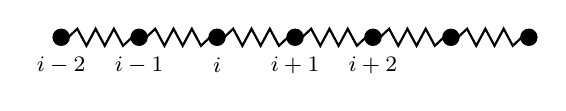
\begin{tikzpicture}[scale=0.9]
  \foreach \i in {0,...,6} {
    \fill (\i*1.1,0) circle (3.5pt);
  }
  \foreach \i in {0,...,5} {
    \draw[thick] (\i*1.1+0.1,0) -- ++(0.128,0.12) -- ++(0.129,-0.24)
      -- ++(0.129,0.24) -- ++(0.129,-0.24) -- ++(0.129,0.24) --
      ++(0.129,-0.24) -- ++(0.127,0.12);
  }
  \node at (0,-0.4) {\footnotesize$i-2$};
  \node at (1.1,-0.4) {\footnotesize$i-1$};
  \node at (2.2,-0.4) {\footnotesize$i$};
  \node at (3.3,-0.4) {\footnotesize$i+1$};
  \node at (4.4,-0.4) {\footnotesize$i+2$};
\end{tikzpicture}
\end{center}

Enfaticemos que el índice $i$ solo nos da el lugar de localización de
los átomos. Supongamos que la cadena es perturbada desplazando los
átomos de su estado de equilibrio, en forma lineal. Sea $q_i$ el
desplazamiento del $i$-ésimo átomo.

\begin{proposicionc}
La ecuación de movimiento del $i$-ésimo átomo es
\[
m\ddot q_i = k(q_{i+1}-q_i) - k(q_i-q_{i-1}) \quad\Longrightarrow\quad
\ddot q_i = \frac{k}{m}\big(q_{i+1}-2q_i+q_{i-1}\big), \qquad
i=1,2,\dots,N.
\]
\end{proposicionc}

\begin{observacion}
Al observar la ecuación de movimiento de la $i$-ésima partícula aparece
un problema en los extremos: si $i=N$, la ecuación involucra $q_{N+1}$,
que no existe (la cadena posee $N$ átomos, no $N+1$); si $i=1$, involucra
$q_0$, que tampoco existe. Los desplazamientos están definidos solo en la
forma $\{q_1,q_2,\dots,q_N\}=\{q_i\}_{i=1}^N$.
\end{observacion}

Para resolver este problema supondremos que la cadena es cerrada en sí
misma, es decir, forma una circunferencia; esto significa que los
desplazamientos satisfacen la condición de \textbf{periodicidad}
\[
q_{i+N} = q_i, \qquad i=1,2,\dots,N.
\]
Con esta condición, $\ddot q_N = \tfrac{k}{m}(q_{N+1}-2q_N+q_{N-1}) =
\tfrac{k}{m}(q_1-2q_N+q_{N-1})$, y análogamente $\ddot q_1 =
\tfrac{k}{m}(q_2-2q_1+q_N)$, de modo que las ecuaciones quedan bien
definidas para todo $i=1,\dots,N$.

\begin{proposicionc}[Lagrangiano de la cadena]
La función Lagrangiana del sistema está dada por
\[
L = \sum_{i=1}^{N} \left(\frac{1}{2}m\dot q_i^2 -
\frac{k}{2}(q_{i+1}-q_i)^2\right),
\]
de la cual se obtiene (ejercicio) la ecuación de movimiento
$\ddot q_i = \tfrac{k}{m}(q_{i+1}-2q_i+q_{i-1})$.
\end{proposicionc}

\section{Cadena continua}

Las ecuaciones anteriores son válidas para sistemas con un número finito
(o numerable) de grados de libertad. Sin embargo, existen problemas con
este formalismo cuando se trata de sistemas continuos, tales como las
vibraciones de un sólido elástico o las del campo electromagnético. El
mecanismo de modificación es tomar el \textbf{límite al continuo}.

Tenemos una cadena unidimensional de átomos discreta y queremos pasar al
continuo: aumentamos el número de átomos sin aumentar el largo de la
cadena. Dado que los átomos están inicialmente a una distancia $h$ unos
de otros, y hay $N$ átomos, el largo de la cadena es $l=Nh$. Si
mantenemos constante $l$ y aumentamos $N$, la separación disminuye:
\[
\left.\begin{aligned} N&\to\infty \\ h&\to 0 \end{aligned}\right\}
\quad\Longrightarrow\quad l = \text{constante}.
\]

Reescribimos la ecuación de movimiento en la forma
\[
\ddot q_i = \frac{k}{m}(q_{i+1}-q_i) - \frac{k}{m}(q_i-q_{i-1}).
\]
En el caso discreto, el índice $i$ identifica a una masa puntual
particular. En el caso continuo, cada punto entre dos átomos contendrá un
átomo nuevo a medida que se agrega un nuevo átomo. De esta forma la
cadena se transforma en una barra, y cada punto de ella queda
determinado por una coordenada de posición $x$, de modo que el índice
$i$ se convierte en $x$:
\[
q_i(t) \to q(t,x), \qquad q_{i+1}(t) \to q(t,x+h), \qquad
\frac{q_{i+1}(t)-q_i(t)}{h} \to \frac{q(t,x+h)-q(t,x)}{h}.
\]

Para pasar al continuo tomamos el límite $h\to 0$:
\[
\lim_{h\to 0} \frac{q(t,x+h)-q(t,x)}{h} = \frac{\partial q(t,x)}{\partial
x}.
\]
Dividiendo la ecuación de movimiento por $h$,
\[
\frac{m}{h}\ddot q_i = k\left(\frac{q_{i+1}-q_i}{h}\right) -
k\left(\frac{q_i-q_{i-1}}{h}\right),
\]
y tomando el límite,
\[
\frac{m}{h}\, \frac{\partial^2 q(t,x)}{\partial t^2} = kh\left(
\frac{q(t,x+h)-q(t,x)}{h^2}\right) - kh\left(\frac{q(t,x)-q(t,x-h)}{h^2}
\right).
\]

Cuando $h\to 0$, el término $m/h$ se convierte en la densidad lineal de
masa $\lambda=dm/dx$. Para el término $kh$ el límite no es evidente. En
una barra elástica que obedece la ley de Hooke, el alargamiento por
unidad de longitud es directamente proporcional a la tensión ejercida
sobre ella, $F=YS$, donde $Y$ es el \textbf{módulo de Young} y
$S=(q_{i+1}-q_i)/h$ es el alargamiento por unidad de longitud. La fuerza
necesaria para estirar el resorte en esta cantidad es
\[
F = k(q_{i+1}-q_i) = kh\left(\frac{q_{i+1}-q_i}{h}\right) = (kh)S,
\]
y tomando el límite, $\lim_{h\to 0} kh = Y$.

\begin{proposicionc}[Ecuación del objeto extendido]
En el límite $h\to 0$,
\[
\lim_{h\to 0}\left[\left(\frac{q(t,x+h)-q(t,x)}{h^2}\right) -
\left(\frac{q(t,x)-q(t,x-h)}{h^2}\right)\right] = \frac{\partial^2
q(t,x)}{\partial x^2},
\]
y se obtiene finalmente
\[
\lambda\, \frac{\partial^2 q(t,x)}{\partial t^2} = Y\, \frac{\partial^2
q(t,x)}{\partial x^2}.
\]
\end{proposicionc}

\begin{proof}
El primer límite es directo, reescribiéndolo como
\[
\lim_{h\to 0} \frac{1}{h}\left[\left(\frac{q(t,x+h)-q(t,x)}{h}\right) -
\left(\frac{q(t,x)-q(t,x-h)}{h}\right)\right] = \lim_{h\to 0}
\frac{1}{h}\left[\frac{\partial q(t,x)}{\partial x} - \frac{\partial
q(t,x-h)}{\partial x}\right] = \frac{\partial^2 q(t,x)}{\partial x^2}.
\]
Sustituyendo $m/h\to\lambda$ y $kh\to Y$ en la ecuación de movimiento se
obtiene el resultado. \qedhere
\end{proof}

Dividiendo por $Y$, el análisis dimensional da $[\lambda/Y] =
\text{s}^2/\text{m}^2$; definimos la velocidad de propagación
$v_p:=\sqrt{Y/\lambda}$, tal que se obtiene la \textbf{ecuación de onda}
\[
\frac{1}{v_p^2}\, \frac{\partial^2 q(t,x)}{\partial t^2} -
\frac{\partial^2 q(t,x)}{\partial x^2} = 0 .
\]

\subsection{El límite de la función Lagrangiana}

Tomemos ahora el límite en la función Lagrangiana:
\[
L = \sum_{i=1}^N \left(\frac12 m\dot q_i^2 - \frac12 k(q_{i+1}-q_i)^2
\right) = \sum_{i=1}^N h\left(\frac12 \frac{m}{h}\dot q_i^2 - \frac12 kh
\left(\frac{q_{i+1}-q_i}{h}\right)^2\right).
\]
Al tomar el límite $h\to 0$ se tiene la correspondencia
\[
h\to dx, \quad q_i(t)\to q(t,x), \quad \frac{m}{h}\to\lambda, \quad
kh\to Y, \quad \sum_{i=1}^N h \to \int dx, \quad \dot q_i(t) \to
\frac{\partial q(t,x)}{\partial t}, \quad \frac{q_{i+1}-q_i}{h} \to
\frac{\partial q(t,x)}{\partial x}.
\]

\begin{proposicionc}
La función Lagrangiana del sistema continuo toma la forma
\[
L = \frac12 \int \left[\lambda\left(\frac{\partial q(t,x)}{\partial
t}\right)^2 - Y\left(\frac{\partial q(t,x)}{\partial x}\right)^2\right]
dx .
\]
\end{proposicionc}

Este simple problema pone de manifiesto las características del
problema general de la transición de un sistema discreto a uno continuo.
Debemos notar que $x$ \textbf{no} es una coordenada generalizada, sino
que es un \textbf{índice continuo} que reemplaza al índice discreto $i$:
del mismo modo que cada valor de $i$ corresponde a una coordenada
generalizada diferente $q_i(t)$, para cada valor de $x$ hay una
coordenada generalizada $q(t,x)$.

\begin{definicion}[Densidad Lagrangiana]
La función Lagrangiana para el caso continuo se escribe como
\[
L = \int \mathscr{L}\left(\frac{\partial q}{\partial t}, \frac{\partial
q}{\partial x}\right) dx, \qquad \mathscr{L}\left(\frac{\partial
q}{\partial t}, \frac{\partial q}{\partial x}\right) = \frac12\left[
\lambda\left(\frac{\partial q(t,x)}{\partial t}\right)^2 -
Y\left(\frac{\partial q(t,x)}{\partial x}\right)^2\right],
\]
donde $\mathscr{L}$ se llama \textbf{densidad Lagrangiana}.
\end{definicion}

\begin{observacion}
La función Lagrangiana posee unidades $[L]=\text{J}=\text{kg}\,
\text{m}^2/\text{s}^2$; la densidad Lagrangiana posee unidades
$[\mathscr{L}] = [L/dx] = \text{J}/\text{m} = \text{kg}\,\text{m}/
\text{s}^2$.
\end{observacion}

\section{Formulación Lagrangiana para sistemas continuos}

Inicialmente comenzamos con una cadena unidimensional cerrada o periódica
y desembocamos, al pasar al continuo, en una densidad Lagrangiana.
Olvidemos que la cadena es cerrada y asumamos un caso más general, es
decir, que tiene bordes en $x=x_i$ y $x=x_f$:
\[
L = \int_{x_i}^{x_f} \mathscr{L}\left(\frac{\partial q}{\partial t},
\frac{\partial q}{\partial x}\right) dx, \qquad \mathscr{L} = \frac12
\left[\lambda\left(\frac{\partial q}{\partial t}\right)^2 -
Y\left(\frac{\partial q}{\partial x}\right)^2\right].
\]
Si $y(t,x)=q(t,x)$ y $T_0=Y$, se recupera la acción de la cuerda
vibrante.

\begin{definicion}[Principio de acción de un sistema continuo]
El \textbf{principio de acción} de un sistema continuo está dado por
\[
S = \int_{t_i}^{t_f} L\, dt = \int_{t_i}^{t_f}\int_{x_i}^{x_f}
\mathscr{L}\left(\frac{\partial q}{\partial t}, \frac{\partial
q}{\partial x}\right) dx\, dt .
\]
\end{definicion}

\begin{observacion}
La variable física $q$ depende de dos coordenadas, $q(t,x)$, y por cada
una de ellas hay una integral en el principio de acción. Esto se resume
diciendo que la densidad Lagrangiana y la acción están relacionadas por
$\mathscr{L} = \partial^2 S/\partial t\,\partial x$.
\end{observacion}

Para obtener la ecuación de campo debemos variar el principio de acción
con respecto a $q$. Del cálculo variacional sabemos que al aplicar la
derivada funcional $\delta/\delta q$ comparamos dos funciones $q(t,x)$
infinitesimalmente cercanas en el espacio de configuración, que en este
caso está dado solo por $q$.

\begin{proposicionc}[Variación de la acción]
La variación de la acción $S=\int_{t_i}^{t_f}\int_{x_i}^{x_f}
\mathscr{L}\,dx\,dt$, con $\mathscr{L}$ como arriba, es
\begin{align*}
\delta S &= \int_{t_i}^{t_f}\int_{x_i}^{x_f} \frac{\delta
\mathscr{L}}{\delta q}\, dx\,dt \\
&\quad + \int_{x_i}^{x_f} \lambda\left[
\frac{\partial q(t_f,x)}{\partial t}\delta q(t_f,x) - \frac{\partial
q(t_i,x)}{\partial t}\delta q(t_i,x)\right] dx \\
&\quad - \int_{t_i}^{t_f} Y
\left[\frac{\partial q(t,x_f)}{\partial x}\delta q(t,x_f) -
\frac{\partial q(t,x_i)}{\partial x}\delta q(t,x_i)\right] dt,
\end{align*}
donde se define la \textbf{derivada funcional} de la densidad
Lagrangiana
\[
\frac{\delta\mathscr{L}}{\delta q} := Y\, \frac{\partial^2 q}{\partial
x^2} - \lambda\, \frac{\partial^2 q}{\partial t^2} .
\]
\end{proposicionc}

\begin{proof}
Aplicando $\delta$ a la acción,
\[
\delta S = \int_{t_i}^{t_f}\int_{x_i}^{x_f} \frac12\left(2\lambda
\frac{\partial q}{\partial t}\delta\frac{\partial q}{\partial t} -
2Y\frac{\partial q}{\partial x}\delta\frac{\partial q}{\partial
x}\right) dx\,dt = \int_{t_i}^{t_f}\int_{x_i}^{x_f}\left(\lambda
\frac{\partial q}{\partial t}\frac{\partial\delta q}{\partial t} -
Y\frac{\partial q}{\partial x}\frac{\partial\delta q}{\partial
x}\right) dx\,dt,
\]
usando que $\delta$ conmuta con las derivadas parciales. Integrando cada
término por partes,
\[
\lambda\frac{\partial q}{\partial t}\frac{\partial\delta q}{\partial t}
= \frac{\partial}{\partial t}\left(\lambda\frac{\partial q}{\partial
t}\delta q\right) - \lambda\frac{\partial^2 q}{\partial t^2}\delta q,
\qquad Y\frac{\partial q}{\partial x}\frac{\partial\delta q}{\partial x}
= \frac{\partial}{\partial x}\left(Y\frac{\partial q}{\partial
x}\delta q\right) - Y\frac{\partial^2 q}{\partial x^2}\delta q,
\]
de donde
\[
\delta S = \int_{t_i}^{t_f}\int_{x_i}^{x_f} \left(Y\frac{\partial^2
q}{\partial x^2} - \lambda\frac{\partial^2 q}{\partial t^2}\right)
\delta q\,dx\,dt + \int_{t_i}^{t_f}\int_{x_i}^{x_f}\left(-\frac{\partial}
{\partial t}\left(\lambda\frac{\partial q}{\partial t}\delta q\right) +
\frac{\partial}{\partial x}\left(Y\frac{\partial q}{\partial x}\delta
q\right)\right) dx\,dt .
\]
Integrando el primer término de borde en $t$ y el segundo en $x$ se
obtiene el resultado. \qedhere
\end{proof}

De la mecánica clásica aprendemos que los extremos temporales de las
trayectorias están fijos; esto lo trasladamos a objetos extendidos y
luego a teoría de campos, de modo que imponemos
\[
\delta q(t_i,x) = \delta q(t_f,x) = 0 .
\]
Para tener un principio de acción bien definido, se debe eliminar
también el término de borde espacial; exigimos, de forma adicional,
\[
\delta q(t,x_i) = \delta q(t,x_f) = 0 .
\]

\begin{proposicionc}[Ecuación de campo]
Imponiendo $\delta S=0$ junto con las condiciones anteriores, se obtiene
\[
\frac{\delta\mathscr{L}}{\delta q} = Y\, \frac{\partial^2 q}{\partial
x^2} - \lambda\, \frac{\partial^2 q}{\partial t^2} = 0,
\]
la ecuación de la cuerda vibrante.
\end{proposicionc}

\begin{observacion}
En la obtención de las ecuaciones de campo no solo se impuso que las
variaciones sean nulas en los extremos temporales, sino que también
deben ser nulas en los extremos espaciales.
\end{observacion}

\subsection{Generalización a la membrana y a tres dimensiones}

Si queremos obtener el principio de acción para una membrana elástica,
\[
S = \int_{t_i}^{t_f}\int_{x_i}^{x_f}\int_{y_i}^{y_f} \frac12\left[
\sigma\left(\frac{\partial z}{\partial t}\right)^2 - Y\vec\nabla z\cdot
\vec\nabla z\right] dx\,dy\,dt, \qquad \vec\nabla z = \ihat
\frac{\partial z}{\partial x} + \jhat\frac{\partial z}{\partial y},
\]
con $\sigma$ la densidad de masa superficial. Variando la acción e
imponiendo que las variaciones se anulen en todos los extremos
(temporales y espaciales),
\[
\delta z(t_i,x,y)=\delta z(t_f,x,y)=0, \quad \delta z(t,x_i,y)=\delta
z(t,x_f,y)=0, \quad \delta z(t,x,y_i)=\delta z(t,x,y_f)=0,
\]
se obtiene $\delta S = \int\int\int (\delta\mathscr{L}/\delta z)\,
dx\,dy\,dt$, con
\[
\frac{\delta\mathscr{L}}{\delta z} = Y\left(\frac{\partial^2 z}
{\partial x^2}+\frac{\partial^2 z}{\partial y^2}\right) - \sigma
\frac{\partial^2 z}{\partial t^2} = Y\nabla^2 z - \sigma\frac{\partial^2
z}{\partial t^2},
\]
y la ecuación de campo $\delta\mathscr{L}/\delta z=0$ es la
\textbf{ecuación de la membrana vibrante}.

Si el objeto extendido es tridimensional se obtiene una ecuación tipo
onda
\[
\nabla^2\phi - \frac{1}{v_p^2}\, \frac{\partial^2\phi}{\partial t^2} =
0,
\]
donde $\phi(t,x,y,z)$ es alguna magnitud física del objeto extendido con
las unidades adecuadas para que $S$ tenga unidades de $\text{J}\cdot
\text{s}$, y $v_p=\sqrt{Y/\rho}$ es la rapidez de propagación, con
$\rho$ la densidad de masa volumétrica.

\section{Ondas planas}

Resolvamos la ecuación de la onda cambiando a las coordenadas
\[
\xi = \vec k\cdot\vec x - \omega t, \qquad \eta = \vec k\cdot\vec x +
\omega t,
\]
con $\vec k$ un vector constante y $\omega$ otra constante. Entonces
\[
\frac{\partial}{\partial t} = \omega\frac{\partial}{\partial\eta} -
\omega\frac{\partial}{\partial\xi} \;\Longrightarrow\; \frac{\partial^2
\phi}{\partial t^2} = \omega^2\left(\frac{\partial^2\phi}{\partial\eta^2}
- 2\frac{\partial^2\phi}{\partial\xi\partial\eta} + \frac{\partial^2
\phi}{\partial\xi^2}\right),
\]
\[
\vec\nabla = \vec k\left(\frac{\partial}{\partial\xi}+\frac{\partial}
{\partial\eta}\right) \;\Longrightarrow\; \nabla^2\phi =
k^2\left(\frac{\partial^2\phi}{\partial\eta^2} + 2\frac{\partial^2
\phi}{\partial\xi\partial\eta} + \frac{\partial^2\phi}{\partial\xi^2}
\right), \qquad k^2 = \vec k\cdot\vec k .
\]
Reemplazando en la ecuación de onda,
\begin{align*}
&k^2\left(\frac{\partial^2\phi}{\partial\eta^2}+\frac{\partial^2\phi}
{\partial\xi^2}\right) - \frac{\omega^2}{v_p^2}\left(\frac{\partial^2
\phi}{\partial\eta^2}-2\frac{\partial^2\phi}{\partial\xi\partial\eta}+
\frac{\partial^2\phi}{\partial\xi^2}\right) = 0 \\
\;\Longrightarrow\;\; &\left(k^2-\frac{\omega^2}{v_p^2}\right)\left(\frac{\partial^2\phi}
{\partial\eta^2}+\frac{\partial^2\phi}{\partial\xi^2}\right) +
2\left(k^2+\frac{\omega^2}{v_p^2}\right)\frac{\partial^2\phi}{\partial
\xi\partial\eta} = 0 .
\end{align*}

\begin{proposicionc}
La solución de la ecuación anterior se obtiene con
\[
k^2 - \frac{\omega^2}{v_p^2} = 0 \;\Longrightarrow\; k=\frac{\omega}
{v_p}, \qquad \frac{\partial^2\phi}{\partial\xi\partial\eta} = 0
\;\Longrightarrow\; \phi(\xi,\eta) = f(\xi)+g(\eta),
\]
con $f$ y $g$ funciones arbitrarias.
\end{proposicionc}

La introducción de $\vec k$ y $\omega$ se debe a que se quiere que
$\xi$ y $\eta$ sean adimensionales: como $[kx]=1$ y $[\omega t]=1$, se
sigue $[k]=1/L$ y $[\omega]=1/T$. El vector $\vec k$ da la dirección de
propagación de la onda, por lo que podemos escribir $\vec k = k\hat n =
(\omega/v_p)\hat n$. Volviendo a coordenadas cartesianas, la solución
general es
\[
\phi(t,\vec x) = f(\vec k\cdot\vec x - \omega t) + g(\vec k\cdot\vec x +
\omega t),
\]
donde $f(\vec k\cdot\vec x-\omega t)$ es una onda que viaja en la
dirección de $+\vec k$, y $g(\vec k\cdot\vec x+\omega t)$ en la
dirección de $-\vec k$. Reemplazando $\vec k=k\hat n$,
\[
\phi(t,\vec x) = f\!\left(\frac{\omega}{v_p}(\hat n\cdot\vec x -
v_pt)\right) + g\!\left(\frac{\omega}{v_p}(\hat n\cdot\vec x + v_pt)
\right).
\]
Si la onda se propaga en la dirección del eje $x$, $\hat n=(1,0,0)$, así
\[
\phi(t,x) = f\!\left(\frac{\omega}{v_p}(x-v_pt)\right) +
g\!\left(\frac{\omega}{v_p}(x+v_pt)\right).
\]

\subsection{Definición de onda plana}

Asumamos por simplicidad que $g=0$, luego $\phi(t,\vec x) = f(\vec
k\cdot\vec x-\omega t)$. Un caso especial importante, que se da en
física (especialmente en electrodinámica), es una onda que viaja en la
dirección $+\vec k$ con la forma
\[
\phi(t,\vec x) = \phi_0\sin(\vec k\cdot\vec x - \omega t),
\]
donde $\phi_0$ es la amplitud de la onda. Este tipo de onda se llama
\textbf{onda plana}.

\begin{proposicionc}
La superficie de fase constante de una onda plana, en un instante fijo,
es un plano perpendicular a $\vec k$.
\end{proposicionc}

\begin{proof}
Por simplicidad analicemos la onda en $t=0$ (el argumento es válido para
cualquier instante), $\phi(0,\vec x) = \phi_0\sin(\vec k\cdot\vec x)$.
Como la función es periódica, existe un punto $\vec x_0$ tal que la onda
se repite espacialmente:
\[
\phi(0,\vec x) = \phi(0,\vec x_0) \;\Longrightarrow\; \sin(\vec
k\cdot\vec x) = \sin(\vec k\cdot\vec x_0) \;\Longrightarrow\; \vec
k\cdot\vec x = \vec k\cdot\vec x_0 + 2\pi n, \quad n\in\mathbb{Z}.
\]
Tomando $n=0$, $\vec k\cdot\vec x = \vec k\cdot\vec x_0
\;\Longrightarrow\; \vec k\cdot(\vec x-\vec x_0) = 0$, que es la
ecuación de un plano perpendicular a $\vec k$. \qedhere
\end{proof}

Como ya se mencionó, la rapidez de propagación $v_p$ es la rapidez con
que la información en el objeto extendido se transmite de un punto a
otro: si en un punto $P$ del objeto extendido oscila, la información que
le indica al punto $Q$ que debe oscilar viaja con rapidez $v_p$.
Volvamos a la cuerda oscilante y consideremos solo la parte que se
propaga en la dirección $+x$, $z(t,x)=f(x-v_pt)$. La rapidez de
oscilación de la cuerda a lo largo del eje $z$ es
\[
\frac{\partial z(t,x)}{\partial t} = \frac{\partial f(x-v_pt)}{\partial
t} = \frac{df}{d\xi}\frac{\partial\xi}{\partial t} = -v_p\frac{df}
{d\xi},
\]
lo que nos dice que la oscilación en el eje $z$ está condicionada a la
propagación de la información en el eje $x$. Por lo tanto, en la cuerda
--y en cualquier objeto extendido-- hay una rapidez máxima, y la
oscilación del objeto está sujeta a ella. Esto está de acuerdo con la
idea de Faraday: hay una velocidad máxima a la que se propagan los entes
físicos, lo que elimina la interacción a distancia o instantánea.

\section{Notación compacta: la métrica de Minkowski}

Volvamos a la cuerda vibrante con el fin de establecer el formalismo
general que luego se usa en teoría de campos. Sea la acción
\[
S = \int_{t_i}^{t_f}\int_{x_i}^{x_f} \frac12\left[\lambda\left(
\frac{\partial z}{\partial t}\right)^2 - T_0\left(\frac{\partial z}
{\partial x}\right)^2\right] dx\,dt .
\]
Reescribiéndola con $T_0=\lambda v_p^2$,
\[
S = \int_{t_i}^{t_f}\int_{x_i}^{x_f} \frac{\lambda v_p^2}{2}\left[
\frac{1}{v_p^2}\left(\frac{\partial z}{\partial t}\right)^2 -
\left(\frac{\partial z}{\partial x}\right)^2\right] dx\,dt .
\]
Definamos $\phi(t,x) := \sqrt{\lambda v_p}\, z(t,x)$, que tiene unidades
$[\phi] = M^{1/2}LT^{-1/2}$. Introduciendo esta variable, la acción se
reduce a
\[
S = \int_{t_i}^{t_f}\int_{x_i}^{x_f} \frac{v_p}{2}\left[\frac{1}{v_p^2}
\left(\frac{\partial\phi}{\partial t}\right)^2 - \left(\frac{\partial
\phi}{\partial x}\right)^2\right] dx\,dt .
\]
Con el fin de hacer notar el paralelismo entre la coordenada temporal y
la espacial, definimos las nuevas coordenadas
\[
x^0 := v_pt \in [x_i^0,x_f^0], \qquad x^1 := x \in [x_i^1,x_f^1],
\]
que tienen la misma dimensión, $[x^0]=[x^1]=L$. Sustituyendo,
\[
S = \int_{x_i^0}^{x_f^0}\int_{x_i^1}^{x_f^1} \frac12\left[
\left(\frac{\partial\phi}{\partial x^0}\right)^2 - \left(\frac{\partial
\phi}{\partial x^1}\right)^2\right] dx^1\,dx^0 .
\]

\begin{definicion}[Métrica de Minkowski en $1+1$ dimensiones]
Se define la matriz simétrica
\[
\eta_{\mu\nu} = \eta_{\nu\mu} = \begin{pmatrix} 1 & 0 \\ 0 & -1
\end{pmatrix}, \qquad \mu,\nu = 0,1,
\]
donde $\mu$ rotula las filas y $\nu$ las columnas.
\end{definicion}

\begin{proposicionc}
\[
\left(\frac{\partial\phi}{\partial x^0}\right)^2 - \left(\frac{\partial
\phi}{\partial x^1}\right)^2 = \eta^{\mu\nu}\, \frac{\partial\phi}
{\partial x^\mu}\, \frac{\partial\phi}{\partial x^\nu} .
\]
\end{proposicionc}

\begin{proof}
\[
\frac{\partial\phi}{\partial x^0}\frac{\partial\phi}{\partial x^0} -
\frac{\partial\phi}{\partial x^1}\frac{\partial\phi}{\partial x^1} =
\eta^{00}\frac{\partial\phi}{\partial x^0}\frac{\partial\phi}{\partial
x^0} + \eta^{11}\frac{\partial\phi}{\partial x^1}\frac{\partial\phi}
{\partial x^1},
\]
y como $\eta^{01}=\eta^{10}=0$, esto es igual a
\[
\eta^{00}\frac{\partial\phi}{\partial x^0}\frac{\partial\phi}{\partial
x^0} + \eta^{01}\frac{\partial\phi}{\partial x^0}\frac{\partial\phi}
{\partial x^1} + \eta^{10}\frac{\partial\phi}{\partial x^1}\frac{
\partial\phi}{\partial x^0} + \eta^{11}\frac{\partial\phi}{\partial
x^1}\frac{\partial\phi}{\partial x^1} = \eta^{\mu\nu}\frac{\partial
\phi}{\partial x^\mu}\frac{\partial\phi}{\partial x^\nu} . \qedhere
\]
\end{proof}

\begin{proposicionc}[Acción compacta]
La acción de la cuerda vibrante toma la forma
\[
S = \frac12\int_{I^0\times I^1} \eta^{\mu\nu}\, \frac{\partial\phi}
{\partial x^\mu}\, \frac{\partial\phi}{\partial x^\nu}\, dx^1\,dx^0,
\qquad I^0=[x_i^0,x_f^0],\quad I^1=[x_i^1,x_f^1].
\]
Definiendo el espacio $M := I^0\times I^1$ (el producto cartesiano
estudiado en el Capítulo~2), la acción se escribe
\[
S = \frac12\int_M \eta^{\mu\nu}\, \frac{\partial\phi}{\partial x^\mu}\,
\frac{\partial\phi}{\partial x^\nu}\, d^2x, \qquad d^2x = dx^1dx^0,
\]
con densidad Lagrangiana $\widetilde{\mathscr{L}} = \tfrac12
\eta^{\mu\nu}(\partial\phi/\partial x^\mu)(\partial\phi/\partial
x^\nu)$, de dimensionalidad $[\widetilde{\mathscr{L}}] =
\text{momento angular}/\text{área} = MT^{-1}$ en el Sistema
Internacional.
\end{proposicionc}

\begin{center}
\begin{tikzpicture}[scale=0.9]
  \draw[-Stealth] (0,0) -- (5,0) node[right] {$x^1$};
  \draw[-Stealth] (0,0) -- (0,3.6) node[above] {$x^0$};
  \draw[fill=colordef!15,draw=colordef] (1,0.7) rectangle (4,2.9);
  \node at (2.5,1.8) {$M=I^0\times I^1$};
  \node at (1,-0.3) {\footnotesize$x_i^1$};
  \node at (4,-0.3) {\footnotesize$x_f^1$};
  \node at (-0.4,0.7) {\footnotesize$x_i^0$};
  \node at (-0.4,2.9) {\footnotesize$x_f^0$};
\end{tikzpicture}
\end{center}

Los principios de acción
\[
S = \int_{t_i}^{t_f}\int_{x_i}^{x_f} \frac12\left[\lambda\left(
\frac{\partial z}{\partial t}\right)^2 - T_0\left(\frac{\partial z}
{\partial x}\right)^2\right] dx\,dt, \qquad S = \frac12\int_M
\eta^{\mu\nu}\, \frac{\partial\phi}{\partial x^\mu}\, \frac{\partial
\phi}{\partial x^\nu}\, d^2x
\]
son equivalentes: la segunda es solo la primera escrita en forma más
compacta.

\subsection{Ecuación de campo en notación compacta}

\begin{proposicionc}
La variación de la acción $S=\tfrac12\int_M \eta^{\mu\nu}
(\partial\phi/\partial x^\mu)(\partial\phi/\partial x^\nu)\, d^2x$ es
\[
\delta S = \int_M \eta^{\mu\nu}\, \frac{\partial\delta\phi}{\partial
x^\mu}\, \frac{\partial\phi}{\partial x^\nu}\, d^2x .
\]
\end{proposicionc}

\begin{proof}
\[
\delta S = \frac12\int_M \left(\eta^{\mu\nu}\delta\frac{\partial\phi}
{\partial x^\mu}\frac{\partial\phi}{\partial x^\nu} + \eta^{\mu\nu}
\frac{\partial\phi}{\partial x^\mu}\delta\frac{\partial\phi}{\partial
x^\nu}\right) d^2x = \frac12\int_M \eta^{\mu\nu}\frac{\partial\delta
\phi}{\partial x^\mu}\frac{\partial\phi}{\partial x^\nu}\, d^2x +
\frac12\int_M \eta^{\mu\nu}\frac{\partial\phi}{\partial x^\mu}
\frac{\partial\delta\phi}{\partial x^\nu}\, d^2x .
\]
En el segundo término renombramos los índices mudos $\mu\leftrightarrow
\nu$ y usamos $\eta^{\nu\mu}=\eta^{\mu\nu}$, con lo que ambos términos
son iguales. \qedhere
\end{proof}

Usando la identidad
\[
\frac{\partial}{\partial x^\mu}\left(\eta^{\mu\nu}\delta\phi\,
\frac{\partial\phi}{\partial x^\nu}\right) = \eta^{\mu\nu}\frac{
\partial\delta\phi}{\partial x^\mu}\frac{\partial\phi}{\partial x^\nu}
+ \eta^{\mu\nu}\frac{\partial^2\phi}{\partial x^\mu\partial x^\nu}
\delta\phi,
\]
se obtiene
\[
\delta S = \int_M \frac{\partial}{\partial x^\mu}\left(\eta^{\mu\nu}
\delta\phi\, \frac{\partial\phi}{\partial x^\nu}\right) d^2x - \int_M
\eta^{\mu\nu}\, \frac{\partial^2\phi}{\partial x^\mu\partial x^\nu}\,
\delta\phi\, d^2x .
\]
La segunda integral corresponde a la ecuación de campo; la primera es el
análogo, en notación compacta, del término de borde del principio de
acción de la mecánica clásica.

\begin{proposicionc}[Teorema de Gauss en notación tensorial]
Recordando el teorema de Gauss, $\int_V \vec\nabla\cdot\vec F\, d^3x =
\int_{\partial V} \vec F\cdot d\vec S$, y usando $\partial V=S$
(Capítulo~3), en notación tensorial se escribe
\[
\int_V \partial_i F^i\, d^3x = \int_{\partial V} F^i\, dS_i,
\]
y su generalización a $n$ dimensiones es
\[
\int_M \partial_i F^i\, d^nx = \int_{\partial M} F^i\, dS_i .
\]
\end{proposicionc}

\begin{definicion}
El elemento de superficie $dS_i$ de $\partial M$, perpendicular a
$\partial M$, es un tensor de orden $(0,1)$.
\end{definicion}

Para nuestro caso,
\[
\int_M \frac{\partial}{\partial x^\mu}\left(\eta^{\mu\nu}\delta\phi\,
\frac{\partial\phi}{\partial x^\nu}\right) d^2x = \int_{\partial M}
\eta^{\mu\nu}\delta\phi\, \frac{\partial\phi}{\partial x^\nu}\, dS_\mu,
\]
con $dS_\mu$ perpendicular a $\partial M$.

\begin{proposicionc}
La variación $\delta\phi$ se anula sobre la frontera $\partial M$ del
rectángulo $M=I^0\times I^1$.
\end{proposicionc}

\begin{proof}
Las condiciones de borde de la cuerda vibrante, $\delta z(t_i,x)=\delta
z(t_f,x)=0$ para $x\in[x_i,x_f]$, y $\delta z(t,x_i)=\delta z(t,x_f)=0$
para $t\in[t_i,t_f]$, se traducen a
\[
\delta\phi(x_i^0,x^1) = \delta\phi(x_f^0,x^1) = 0 \ \text{ para }
x^1\in I^1, \qquad \delta\phi(x^0,x_i^1) = \delta\phi(x^0,x_f^1) = 0 \
\text{ para } x^0\in I^0 .
\]
Usando la notación de producto cartesiano, la primera condición se
escribe $\delta\phi=0$ sobre $\big(\{x_i^0\}\cup\{x_f^0\}\big)\times
I^1$, y la segunda, $\delta\phi=0$ sobre $I^0\times\big(\{x_i^1\}\cup
\{x_f^1\}\big)$. Por lo tanto,
\[
\delta\phi = 0 \ \text{ sobre } \ \big(\{x_i^0\}\cup\{x_f^0\}\big)
\times I^1 \ \cup \ I^0\times\big(\{x_i^1\}\cup\{x_f^1\}\big) =
\partial I^0\times I^1 \ \cup \ I^0\times\partial I^1 =
\partial(I^0\times I^1) = \partial M,
\]
usando el resultado del Ejemplo~3.10.1 (frontera de un rectángulo,
Capítulo~3). \qedhere
\end{proof}

Como $\delta\phi=0$ sobre $\partial M$, el término de borde se anula,
\[
\int_M \frac{\partial}{\partial x^\mu}\left(\eta^{\mu\nu}\delta\phi\,
\frac{\partial\phi}{\partial x^\nu}\right) d^2x = \int_{\partial M}
\eta^{\mu\nu}\delta\phi\, \frac{\partial\phi}{\partial x^\nu}\, dS_\mu =
0,
\]
de modo que la variación de la acción se reduce a
\[
\delta S = -\int_M \eta^{\mu\nu}\, \frac{\partial^2\phi}{\partial
x^\mu\partial x^\nu}\, \delta\phi\, d^2x .
\]

\begin{proposicionc}[Ecuación de campo compacta]
Imponiendo el principio variacional $\delta S=0$ se obtiene
\[
\eta^{\mu\nu}\, \frac{\partial^2\phi}{\partial x^\mu\partial x^\nu} = 0
.
\]
\end{proposicionc}

\begin{observacion}[Resumen]
El principio de acción de la cuerda vibrante se escribió en dos formas:
\[
\begin{array}{ll}
\textbf{Original:} & S = \displaystyle\int_{t_i}^{t_f}\int_{x_i}^{x_f}
\frac12\left[\lambda\left(\frac{\partial z}{\partial t}\right)^2 -
T_0\left(\frac{\partial z}{\partial x}\right)^2\right] dx\,dt, \qquad
\dfrac{1}{v_p^2}\dfrac{\partial^2 z}{\partial t^2} - \dfrac{\partial^2
z}{\partial x^2} = 0. \\[10pt]
\textbf{Compacta:} & S = \displaystyle\frac12\int_M \eta^{\mu\nu}\,
\frac{\partial\phi}{\partial x^\mu}\frac{\partial\phi}{\partial x^\nu}\,
d^2x, \qquad \eta^{\mu\nu}\, \dfrac{\partial^2\phi}{\partial x^\mu
\partial x^\nu} = 0.
\end{array}
\]
\end{observacion}

\section{Condiciones de borde}

En la obtención de las ecuaciones de campo aparece la integral de borde
\[
\int_M \frac{\partial}{\partial x^\mu}\left(\eta^{\mu\nu}\delta\phi\,
\frac{\partial\phi}{\partial x^\nu}\right) d^2x = \int_{\partial M}
\eta^{\mu\nu}\delta\phi\, \frac{\partial\phi}{\partial x^\nu}\, dS_\mu,
\]
y lo que se hace con ella es tratar de eliminarla de la variación de la
acción. Con este fin, se imponen algunas condiciones a los campos en el
borde $\partial M$.

\begin{definicion}[Condición de borde de Dirichlet]
Se especifica un valor único de los campos en todos los puntos de la
frontera. Por ejemplo, en una lámina cuadrada con una distribución de
temperatura, podemos fijar el borde a temperatura $0\,^\circ$C.
\end{definicion}

Para el caso que estudiamos, la condición de Dirichlet conduce a
$\delta\phi=0$ sobre $\partial M$, y entonces el término de borde
satisface
\[
\int_M \frac{\partial}{\partial x^\mu}\left(\eta^{\mu\nu}\delta\phi\,
\frac{\partial\phi}{\partial x^\nu}\right) d^2x = \int_{\partial M}
\eta^{\mu\nu}\delta\phi\, \frac{\partial\phi}{\partial x^\nu}\, dS_\mu =
0 .
\]

\begin{definicion}[Condición de borde de Neumann]
Se especifica un valor único para la derivada de los campos en todos los
puntos de la frontera. Por ejemplo, en dinámica de fluidos se fija el
flujo de entrada o salida en el borde de un sistema.
\end{definicion}

Para nuestro caso, la condición de Neumann conduce a
$\delta(\partial\phi/\partial x^\mu)=0$ sobre $\partial M$, y entonces
el término de borde \textbf{no} se anula en general,
\[
\int_M \frac{\partial}{\partial x^\mu}\left(\eta^{\mu\nu}\delta\phi\,
\frac{\partial\phi}{\partial x^\nu}\right) d^2x = \int_{\partial M}
\eta^{\mu\nu}\delta\phi\, \frac{\partial\phi}{\partial x^\nu}\, dS_\mu
\neq 0 .
\]

\begin{observacion}
En este caso el término de borde no se anula, lo que genera un problema:
se debe eliminar esta integral de borde modificando el principio de
acción $S$. Lo que se hace es adicionar una nueva integral a la acción
original, $S'=S+B$, tal que $B$ satisfaga
\[
\int_{\partial M} \eta^{\mu\nu}\delta\phi\, \frac{\partial\phi}
{\partial x^\nu}\, dS_\mu + \delta B = 0,
\]
lo que permite inferir cómo debe ser $B$. Este caso no se estudia en
este curso.
\end{observacion}

\begin{definicion}[Condiciones de borde de Robin]
Especifican una combinación lineal de las condiciones de borde de
Dirichlet y de Neumann en el borde. No se estudian en este curso.
\end{definicion}

\section{Conclusiones}

Después de un largo trabajo matemático se obtuvo un formalismo para los
llamados \textbf{Lagrangianos continuos}. Se introdujeron importantes
conceptos matemáticos que dan solidez al formalismo. Pero uno de los
conceptos más importantes que se introduce es que en los Lagrangianos
continuos existe una \textbf{rapidez máxima} de propagación.

¿Existe una velocidad máxima en la naturaleza? La respuesta es: sí.

